\documentclass[oneside]{Tptesi}
\usepackage[]{babel}
\usepackage[T1]{fontenc} % Usa la nuova codifica standard dei caratteri in LaTeX
\usepackage{graphicx}
\usepackage{rotating}
\usepackage{minted}
\usepackage{eurosym}
\usepackage{float}
\usepackage{hyperref}
\usepackage{amsfonts}
\usepackage{amsmath}
\usepackage{cite}
\usepackage{caption}
\usepackage{subcaption}
\usepackage{cleveref}
\newcommand\Chapter[2]{
  \chapter[#1: {#2}]{#1\\[2ex]\Large#2}
}
\newminted{rb}{baselinestretch=auto,tabsize=4,fontsize=\footnotesize,frame=lines,samepage=true}
\usepackage{pifont}
\usepackage{epstopdf}
\usepackage[italian]{varioref}
\usepackage[utf8]{inputenc}
\usepackage{graphicx}
\usepackage[export]{adjustbox}[2011/08/13]
\usepackage{caption}
\usepackage{subcaption}
\usepackage{booktabs} 
\usepackage{multirow}
\usepackage{url}
\hypersetup{urlcolor=black}
\usepackage{imakeidx}
\makeindex[title=Ciao]
				
% ------------------------------------------------------------------------------
% Metadata (Change this)
% ------------------------------------------------------------------------------
	\title{Disparity coherent stereo video watermarking}
	\author{Benedetta Barbetti, Michaela Servi}
	\titolocorso{Computer Engineering}
	\chair{Prof. Alessandro Piva}
	\numberofmembers{1} %numero dei relatori
	\othermembers{Prof. Paolo Nesi}
	\degreeyear{2014/2015}
	\numerocorrelatori{2} %numero dei correlatori
	\correlatori{Prof. Carlo Colombo\\ Dott. Pasquale Ferrara\\Dott. Francesca Uccheddu} 
	\dataTesi{December 2015}



% ---- Inclusioni separate da virgole e senza spazi  --------------
\includeonly 
{abstract, introduction, stereo_video, watermark, doer, dft, conclusions, bibliografia}
%
%%//// document ///////////////////////////////////////////////////////////////

\begin{document}
\hyphenation{}
%
%
\maketitle % crea il frontespizio(ricordati di copiare "stemma.eps" nella tuadirectory)%

\thispagestyle{empty}
\begin{flushright}
\large\em \vspace*{2cm}

   
\end{flushright}

%----- Abstract
\begin{abstract}
Nowdays stereoscopic videos play an important role in many applications: from medical diagnosis and endoscopic surgery to fault detection in manufactory industry, army and arts, in people tracking and mobile robotics navigation as, naturally, in the film industry with 3D movie release.\\
The huge increase of distribution systems of this content leads to the increase of concerns over content copyright protection: in this thesis a blind disparity-coherent watermarking technique has been presented to protect stereoscopic video contents.\\
The algorithm belongs to view-based methods and operates in both frequency and spatial domain in a diparity-coherent way, namely, a physical point of the captured scene always carries the same watermark sample regardless of where it appears in the left and right views.\\
This kind of techniques has been proved to yield less visual discomfort and to be robust against view synthesis attacks, as shown by the experiments conducted on the implemented algorithm.


\end{abstract}
% --- Crea la pagina dei ringraziamenti (se ti va) ---

%% --- Fine ringraziamenti ----------------
%%
\pagenumbering{arabic}
\pagestyle{plain}
\tableofcontents % inserisce indice generale
\listoffigures   % inserisce indice figure
\listoftables    % inserisce indice tabelle
%\listoflistings	 % inserisce indice di codici
%%
%%--------------- Inizio del testo vero e proprio
%%

\cleardoublepage
\pagenumbering{arabic}
\pagestyle{headings}

%% ////////////////////////////////////////////////////////////////////////////
\chapter*{Introduction}
\markright{Introduction}
\label{intro}
\phantomsection
\addcontentsline{toc}{chapter}{Introduction}

In the last few years the stereoscopic technique has become a great part of image and video processing.\\
In medical diagnosis and endoscopic surgery as in fault detection in manufactory industry, army and arts,
multiview imaging is considered as a key enabler  for professional added value services.\\
Nowdays stereoscopic techniques are also used in people tracking and mobile robotics
navigation for economic reasons and to improve performances.\\
Finally the worldwide success of 3D movie releases and 3D video games and the deployment of 3D televisions made the nonprofessional user aware about a new type of multimedia entertainment experience.\\
The increasing production and distribution of these contents leads to the concerns over copyright protection.\\
Digital watermarking can be considered as the most flexible property right protection technology, since it adds some information (a mark, i.e. copyright information) in the
original content without altering its visual quality so that such a marked content can be further distributed/consumed by another user without any restriction; still, the legitimate/illegitimate usage can be determined at any moment by detecting the mark. In same case the watermarking protection mechanism, instead of restricting the media copy/distribution/consumption, provides means for tracking the source of the content illegitimate usage.\\
The purpose of this thesis is to provide a new watermarking system for copyright protection of stereoscopic videos. The method operates in the frequency and in the spatial domain by embedding a pseudo-random sequence of real numbers in a selected set of DFT coefficients of the left image; then the reference watermark is distorted according to the depth information prior to insertion and spatially added to the right image.\\
In Chapter \ref{}...
\chapter{Stereoscopic Video}
\markright{Stereoscopic Video}
\label{stereo_video}
\phantomsection
%\addcontentsline{toc}{chapter}{Stereoscopic Video}

In a wide variety of image processing applications, explicit depth information is required in
addition to general image informations, such as intensities, color, densities.\\
Examples of such applications are found in 3D vision (robot vision, photogrammetry, remote sensing systems), in medical imaging (computer tomography,
magnetic resonance imaging, microsurgery), in remote handling of objects (random bin picking), in space exploration (mobile robotics navigation) or 3D movies and videogames.\\
In each of these cases, depth information is essential for accurate image analysis or for enhancing the
realism.\\
In remote sensing the terrain's elevation needs to be accurately determined for map production, in remote handling an operator needs to have precise knowledge of the threedimensional organization of the area to avoid collisions and misplacements.\\
\begin{figure}[h!]
\centering
\begin{subfigure}[]{0.5\textwidth}
		\centering
        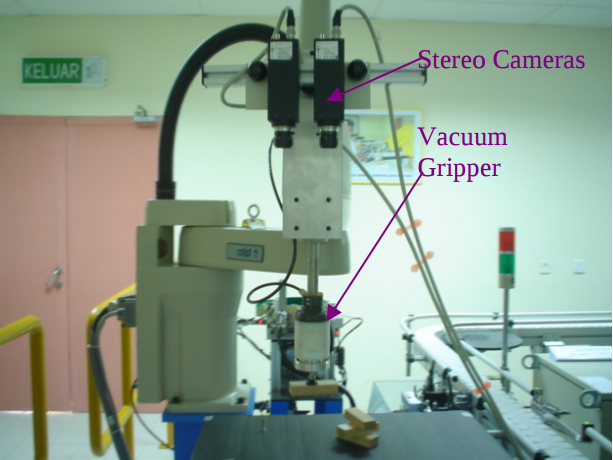
\includegraphics[width=0.7\textwidth]{./img/bin_pick.png}
                \caption{\scriptsize{In bin picking applications stereo vision helps to reconstruct the 3D environment and detect the part of the object to be robotically picked}}
\end{subfigure}% 
~ \quad
\begin{subfigure}[]{0.5\textwidth}
	\centering
	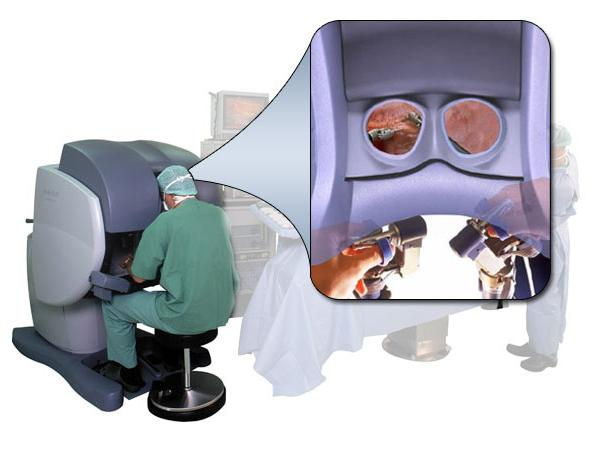
\includegraphics[width=0.7\textwidth]{./img/da_vinci.jpg}
          \caption{\scriptsize{Surgical robot \textit{Da vinci} is provided with a stereoscopic camera that allows a tridimensional view of the operative filed.}}
\end{subfigure} 
\caption{\small{Stereoscopy in medical and industrial field}}
\end{figure}

\begin{figure}[h!]
\centering
\begin{subfigure}[]{0.5\textwidth}
		\centering
        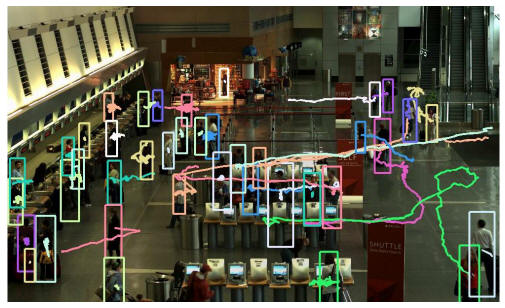
\includegraphics[width=0.7\textwidth]{./img/tracking.jpg}
                \caption{\scriptsize{In people tracking application stereo vision improves segmentation thanks to depth information and it's less sensible to light changes.}}
\end{subfigure}% 
~ \quad
\begin{subfigure}[]{0.5\textwidth}
		\centering
        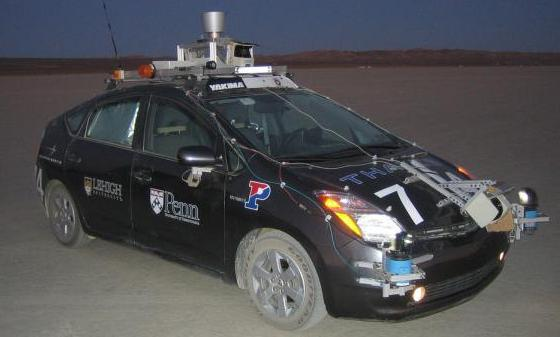
\includegraphics[width=0.7\textwidth]{./img/little_ben.jpg}
                \caption{\scriptsize{In mobile robotics navigation stereo vision has became the first choice technology because it provids a lot of quality data for low costs.}}
\end{subfigure} 
\caption{\small{Stereoscopy application's fields}}
\end{figure}
Depth in real world scenes can be explicitly measured by a number of range sensing devices such as by laser range sensors, by structured light or by ultrasound.
However it's usually undesirable to have separate systems for acquiring the intensity and the depth
information because of the relative low resolution of the range sensing devices and because it's not an easy task to fuse information from different type of sensors; for these reasons and for a non-negligible economic factor stereoscopic vision has becoming the technology of choice in these type of applications.
\begin{figure}[h!]
\centering
\begin{subfigure}[]{0.4\textwidth}
		\centering
        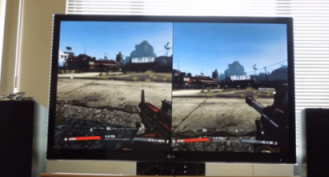
\includegraphics[width=0.7\textwidth]{./img/games1.png}
                \caption{\scriptsize{Stereo video frames, left and right.\newline}}
\end{subfigure}
\begin{subfigure}[]{0.4\textwidth}
		\centering
        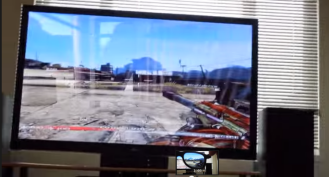
\includegraphics[width=0.7\textwidth]{./img/games2.png}
                \caption{\scriptsize{Overlap of the two frames.}}
\end{subfigure} 
\begin{subfigure}[]{0.4\textwidth}
		\centering
        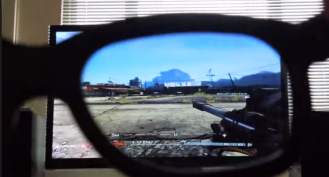
\includegraphics[width=0.7\textwidth]{./img/games3.png}
                \caption{\scriptsize{3D view with specific glasses}}
\end{subfigure}%
\begin{subfigure}[]{0.4\textwidth}
		\centering
        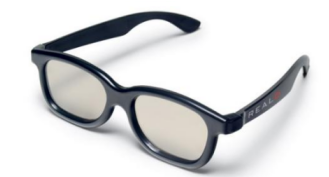
\includegraphics[width=0.7\textwidth]{./img/games4.png}
                \caption{\scriptsize{Polarized glasses for 3D view}}
\end{subfigure} 
\caption{\small{Stereoscopy in 3D video games}}
\end{figure}

\section{Stereo vision}
In image processing stereo vision is the process of extracting 3D information from multiple 2D views of a scene. \\
The 3D information can be obtained from a pair of images, also known as a stereo pair, by estimating the relative depth of points in the scene.\\
From the anatomic point of view, the human brain calculates the depth in a visual scene mainly by
processing the information brought by the images seen by the left and the right eyes. These left and right images are slightly different because the eyes have biologically different emplacements.\\
Consequently, the straightforward way of achieving stereoscopic digital imaging is to emulate the
Human Visual System (HSV) by setting-up (under controlled geometric positions), two traditional 2D
cameras.\\
\begin{figure}[h]
\centering
\begin{subfigure}[b]{0.35\textwidth}
        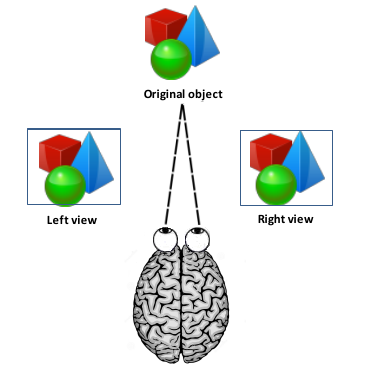
\includegraphics[width=\textwidth]{./img/hvs.png}
         \caption{\scriptsize{Binocular human visual system}}
         \label{fig:hvs}
\end{subfigure}
\begin{subfigure}[b]{0.35\textwidth}
        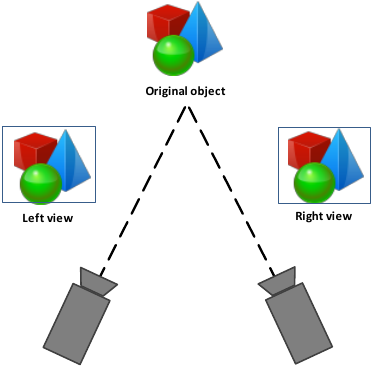
\includegraphics[width=\textwidth]{./img/stereo.png}
        \caption{\scriptsize{Stereoscopic system}}
        \label{fig:stereo}
\end{subfigure} 
\caption{\small{Binocular human vision vs. stereoscopic content acquisition.}}
\end{figure}

\subsection{Acquisition of stereoscopic images}\label{sec:acquisition-of-stereoscopic-images}

In order to be able to perceive depth using recorded images, a stereoscopic camera is required,
which consists of two cameras that capture two different, horizontally shifted perspective
viewpoints; with two (or more) cameras we can infer depth, by means of triangulation, if we are able to find corresponding points in the two images (Figure).\\
\begin{figure}[h!]
\centering
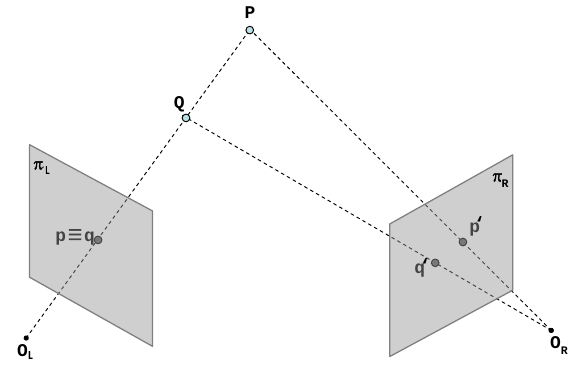
\includegraphics[width=0.6\textwidth]{./img/correspondance.png}
\caption{\small{Triangulation: with two cameras the depth of }}
\label{fig:corr}
\end{figure}
 The camera setup should be geometrically
calibrated such that the two cameras capture the same part of the real world scene.\\
Calibration of a stereo camera system involves the estimation of the intrinsic and extrinsic parameters of the model: intrinsic parameters embody the characteristics of the optical system and its geometric relationship with the image sensor, extrinsic parameters relate the location and orientation of the second camera with respect to the first one in the 3D space (Figure).\\
\begin{figure}[h!]
\centering
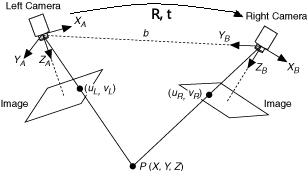
\includegraphics[width=0.6\textwidth]{./img/stereo_system.png}
\caption{\small{Stereo camera model}}
\label{fig:rt}
\end{figure}
These parameters can be used to rectify a stereo pair of images to make them appear as the two image planes are parallel (Figure); once the images are rectified, epipolar geometry it's used to find corresponding points and compute the disparity map.\\
\begin{figure}[h!]
\centering
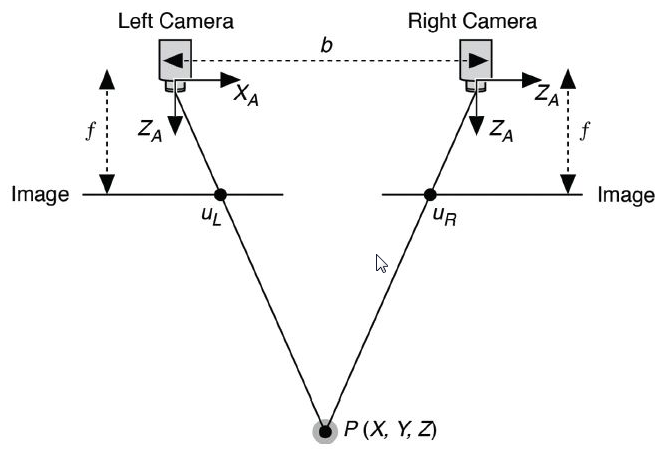
\includegraphics[width=0.6\textwidth]{./img/rect_stereo.png}
\caption{\small{Rectified stereo cameras}}
\label{fig:rect_stereo}
\end{figure}
\begin{figure}[h!]
\centering
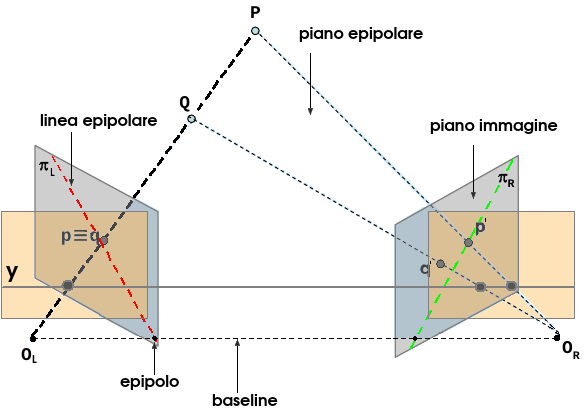
\includegraphics[width=0.6\textwidth]{./img/standard.png}
\caption{\small{Rectified images: corresponding points (p, p'), projection of the same 3D point (P) are constrained on the same image horizontal line, the epipolar line}}
\label{fig:std}
\end{figure}

\newpage
\subsection{Disparity map computation}

With the stereo rig in standard form and by considering similar triangles in Figure XX (PO$_{L}$O$_{R}$ and Ppp'): 
$$
\frac{b}{Z} = \frac{(b+x_{L}) - x_{R}}{Z-f} 
$$ 
so
$$
Z = \frac{b \cdot f}{x_{L} - x_{R}} = \frac{b \cdot f}{d}
$$ 

where $ d = x_{L} - x_{R} $ it's called \textit{disparity}.\\
\begin{figure}[h!]
\centering
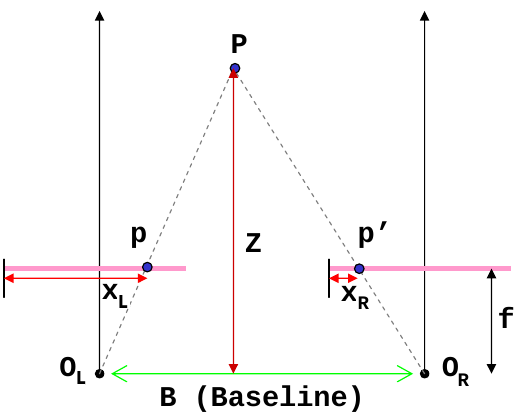
\includegraphics[width=0.6\textwidth]{./img/depth.png}
\caption{\small{Geometry of standard form}}
\label{fig:depth}
\end{figure}
Disparity is, therefore, the difference between the $x$ coordinates of two corresponding points and it is usually encoded with greyscale image (Figure XX), where points closer to the cameras are brighter and correspond to a higher disparity.\\
\begin{figure}[h!]
\centering
\begin{subfigure}[]{0.4\textwidth}
\centering
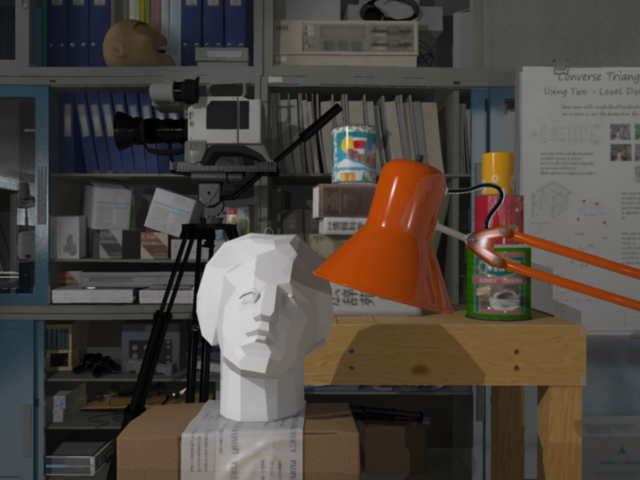
\includegraphics[width=0.7\textwidth]{./img/left.png}
\caption{\scriptsize{Left image}}
\end{subfigure}% 
~ %add desired spacing between images, e. g. ~, \quad, \qquad, \hfill etc.$  $
  %(or a blank line to force the subfigure onto a new line)
\begin{subfigure}[]{0.4\textwidth}
\centering
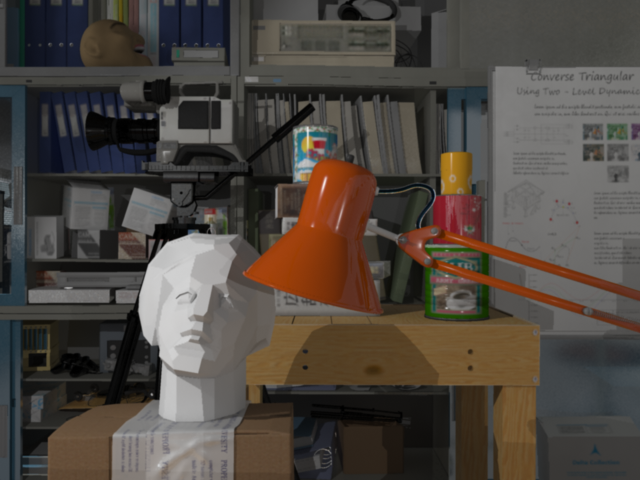
\includegraphics[width=0.7\textwidth]{./img/right.png}
\caption{\scriptsize{Right image}}
\end{subfigure} 
~\quad
\begin{subfigure}[]{0.4\textwidth}
\centering
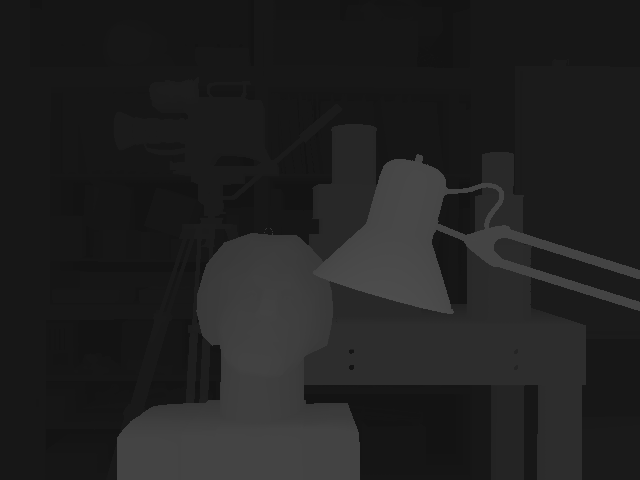
\includegraphics[width=0.7\textwidth]{./img/disparity.png}
\caption{\scriptsize{Disparity map}}
\label{disparity}
\end{subfigure}%
\caption{\small{Stereo pair and disparity map}}
\end{figure}
In order to compute the disparity map is necessary to find corresponding points; stereo correspondance is though a challenging task that has to manage with perspective distortions, uniform and ambiguous regions, repetitive patterns, occlusions and discontinuities(Figure XX).\\
\begin{figure}[h!]
\centering
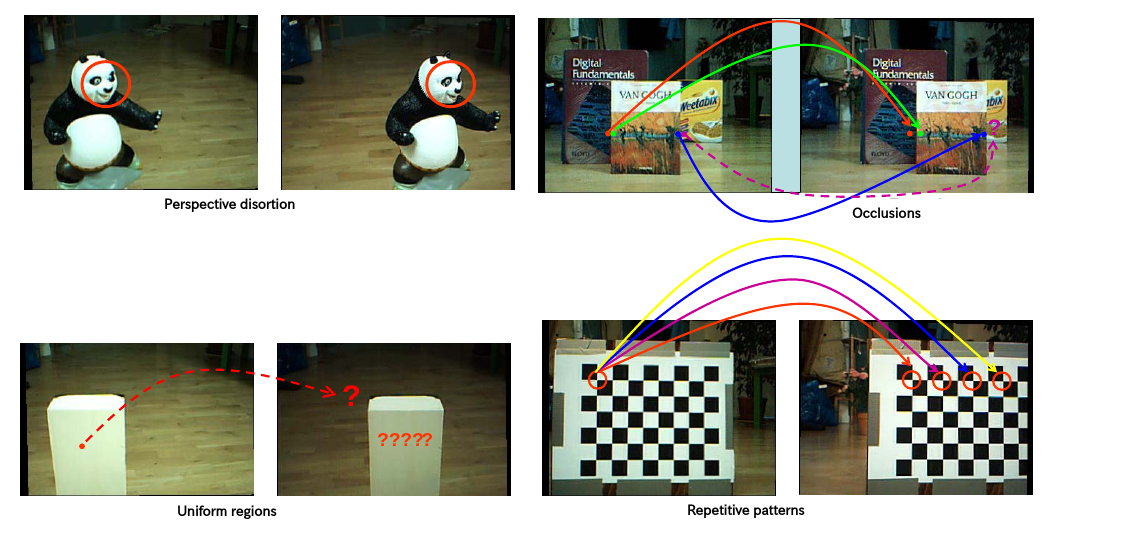
\includegraphics[width=0.6\textwidth]{./img/occl.png}
\caption{\small{Stereo matching general problems}}
\label{fig:occl}
\end{figure}
In general, stereo matching algorithms can be categorized into two major classes:
\begin{itemize}
\item local methods
\item global methods.
\end{itemize}
Local stereo algorithms estimate the correspondence using a local support region or a window. Local algorithms generally rely on an approximation of the smoothness constraint assuming that all pixels within the matching region have the same disparity. However, this assumption is not valid for highly curved surfaces or around disparity discontinuities.\\
A naive approach consists of comparing each  pixel or window in the left image with every pixel or window on the same epipolar line in right image and picking position with minimum match cost (e.g., SSD, SAD, normalized correlation).\\ 
\begin{figure}[h!]
\centering
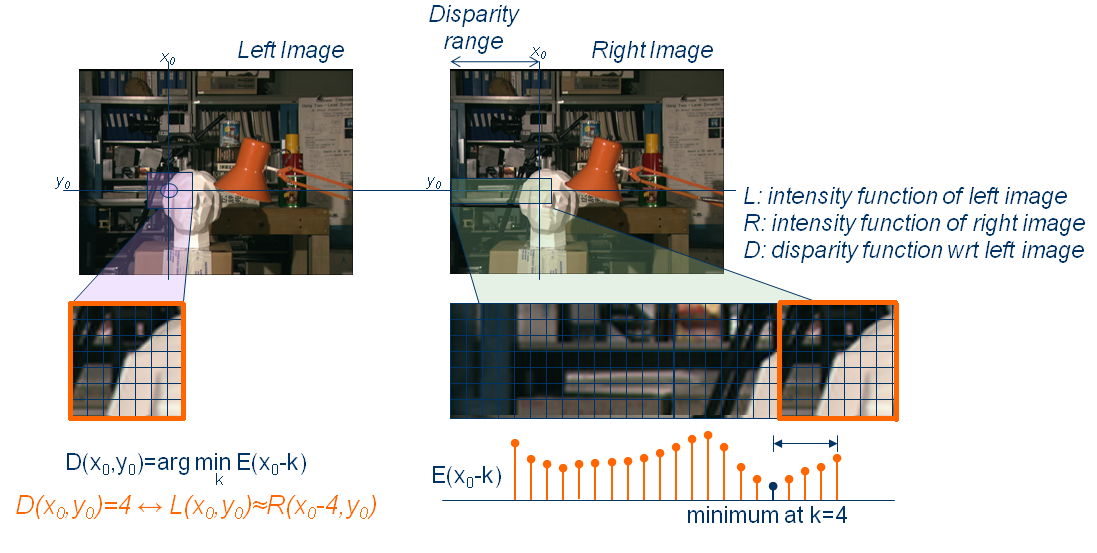
\includegraphics[width=0.7\textwidth]{./img/local.png}
\caption{\small{Local stereo matching, window based}}
\label{fig:local}
\end{figure}
Global stereo methods consider stereo matching as a labeling problem where the pixels of the reference image are nodes and the estimated disparities are labels. An energy functional embeds the matching assumptions by its data, smoothness, and occlusion terms and propagates them along the scan line or through the whole image. The labeling problem is solved by energy functional minimization, using dynamic programming, graph cuts, or belief propagation.\\
Even if this class of algorithms is significantly slow, the results, especially when textures and discontinuities are present, are much accurate.\\
\newline
In this thesis the Kolmogorov and Zabih's Graph Cuts Stereo Matching Algorithm has been used, because there were no time constraints requirements and the quality of the computed disparities has been considered satisfying regard to the ground trouth.\\








\section{Acquisition of stereo images}


\section{Display 3D video}

\chapter{Stereo video watermarking}
\markright{Stereo video watermarking}
\label{wat}
\phantomsection
%\addcontentsline{toc}{chapter}{Stereoscopic Video}

\section{Watermaking}

Digital watermarking consists in imperceptiby and persistently associating some extra information with some original content. \\
The basic watermarking workflow is presented in Figure \ref{fig:workflow}.\\
\begin{figure}[h!]
\centering
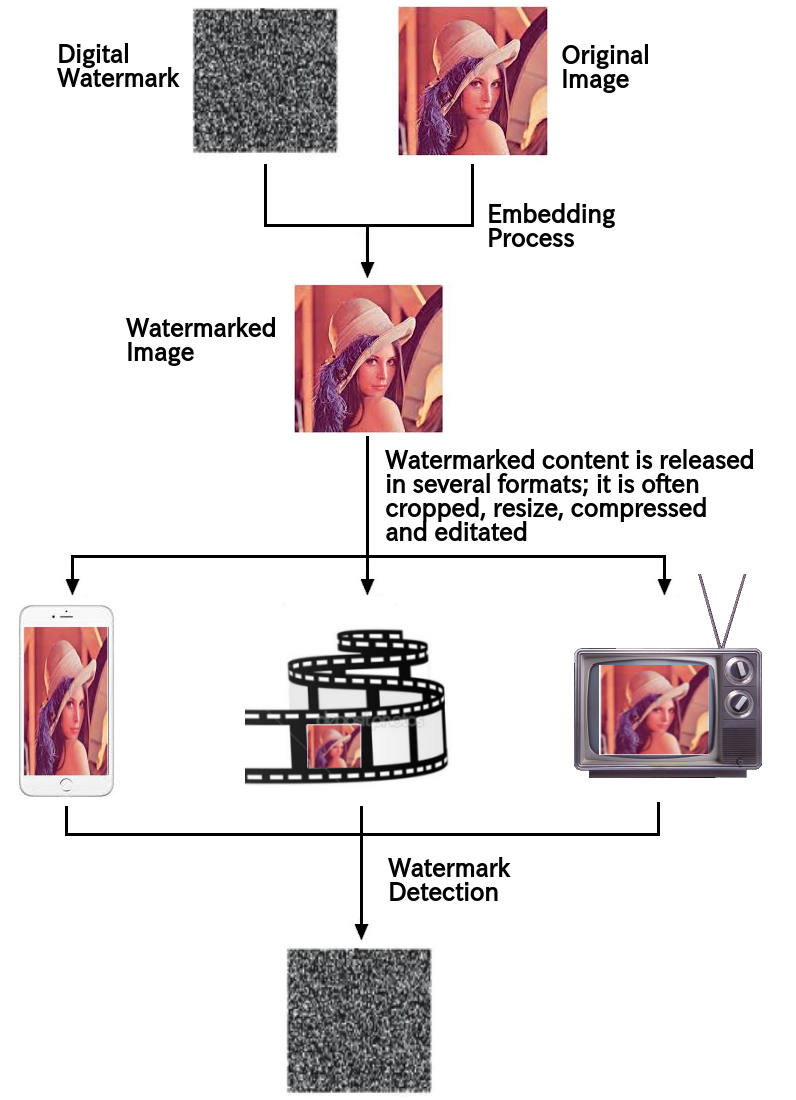
\includegraphics[width=0.6\textwidth]{./img/wat_workflow.png}
\caption{\small{Watermarking workflow}}
\label{fig:workflow}
\end{figure}
\clearpage
\subsection{Properties}
Three parameters are required to evaluate watermarking technique performances:
\begin{itemize}
\item[-] perceptual impact, that is the misure of how much the watermark affects the quality of the host data;
\item[-] robustness, i.e.,the capability of the hidden data to survive host signal manipulation including compression, signal processing, geometric manipulations;
\item[-] data payload, that is the amount of data of information bits that it is able to convey.
\end{itemize}
These requirements are though inversely proportional (Figure \ref{fig:properties}): the more information is embedded, the more the watermark is visible and viceversa; the more robusteness is encreased, the more the watermark is visible and viceversa.\\
\begin{figure}[h!]
\centering
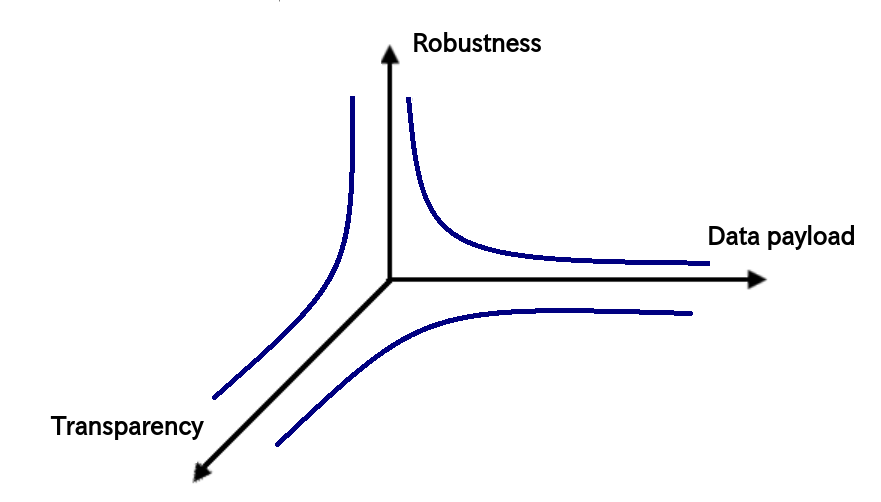
\includegraphics[width=0.4\textwidth]{./img/properties.png}
\caption{\small{Watermark properties trade-off}}
\label{fig:properties}
\end{figure}
Finally, a watermarking technique can be:
\begin{itemize}
\item[-] non-blind/blind, if at the decoder side the original content is available or not, respectively;
\item[-] private/public if only authorized users
can recover it or if anyone to read the watermark, respectively;
\item[-] detectable/readable, if it is only possible to decide whether a given watermark is embedded in the content or if the bits hidden in the content can be read without knowing them in advance, respectively.
\end{itemize}




\subsection{Embedding domains}
Host features modified during embedding can
belong to 
\begin{itemize}
\item[-] spatial domain: the watermark is embedded by directly modifying the pixel values;
\begin{figure}[h!]
\centering
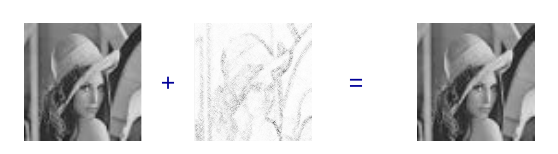
\includegraphics[width=1\textwidth]{./img/domain1.png}
\caption{\small{Spatial domain watermark insertion}}
\label{fig:dom1}
\end{figure}
\item[-] frequency domain: the image is transformed through a mathematical transformation, some coefficients are modified and finally the inverse transform is carried out;
\begin{figure}[h!]
\centering
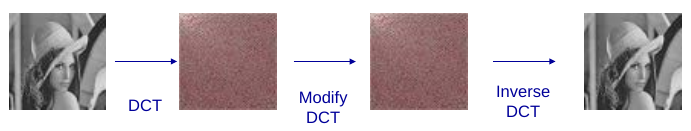
\includegraphics[width=1\textwidth]{./img/domain2.png}
\caption{\small{Frequency domain watermark insertion}}
\label{fig:dom2}
\end{figure}
\item[-] hybrid techniques: a block wise transform is applied, the image is divided
into blocks and for each block a mathematical transformation is computed, some coefficients are modified and the inverse transform is done.
\begin{figure}[h!]
\centering
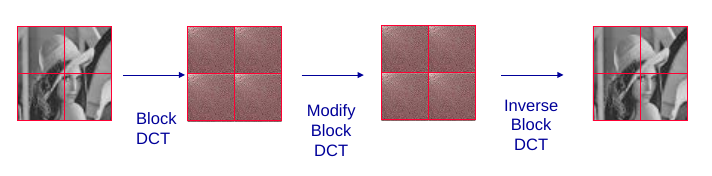
\includegraphics[width=1\textwidth]{./img/domain3.png}
\caption{\small{Hybrid technique}}
\label{fig:dom3}
\end{figure}
\end{itemize}

\subsection{Embedding techniques}
The most straightforward ways to add a watermark in a given content have been proved to be Spread Spectrum (SS) approach and Side Information (SI).\\
\begin{figure}[h!]
\centering
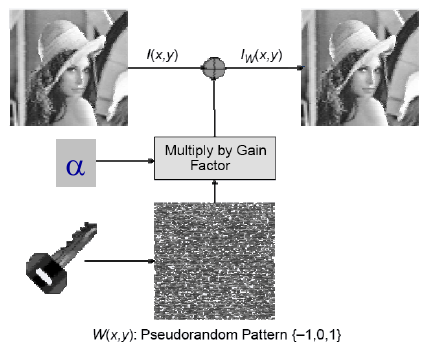
\includegraphics[width=0.6\textwidth]{./img/ss.png}
\caption{\small{Spread spectrum technique}}
\label{fig:ss}
\end{figure}
As in spread spectrum communications, the former approach considers the original content as a signal and the watermark as a noise that is spread over very many frequency bins so that the energy in any one bin is very small and certainly undetectable\cite{COX}\cite{COX1}.\\
The latter takes advantage of the fact that the original content is known at the embedder side (but unknown at the detector): this way the watermark can be modulated  according to the original and the quantity of inserted data can be maximed\cite{COX2,SH, EG, COSTA}.\\

Sometimes hybrid watermarking methods combining spread spectrum and side information concepts can be applied; they try to benefit from both the robustness and transparency of the spread spectrum methods and the increased data payload of the side information methods \cite{QIM}\cite{QIM1}.
\begin{figure}[h!]
\centering
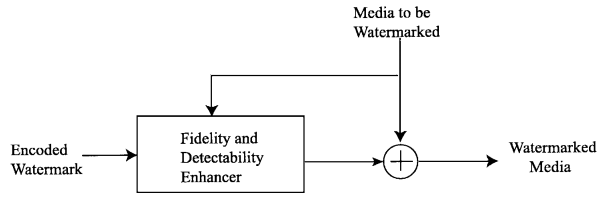
\includegraphics[width=0.7\textwidth]{./img/si.png}
\caption{\small{Side information technique scheme}}
\label{fig:si}
\end{figure}

\section{Stereoscopic video watermarking}

In the literature, stereoscopic video watermarking has been initially approached as a direct extension of still image watermarking, i.e. by considering the right and the left views as two independent images. This way, the stereo data can be straightforward exploited with basic 2D methods. However, such straightforward application does not consider the peculiarities of the stereoscopic video content, therefore a second modality considers derived representations from the stereo pair, as a disparity map.\\ 
A new approach, however, has been recently introduced in stereoscopic view-based methods: disparity-coherent watermarking \cite{DOER}.

\subsection{Embedding domain}
In stereoscopic video context the studies can be structured in two other categories in addition to spacial and frequency domain:
\begin{itemize}
\item[-] view-based methods \cite{16,17,18,19,20,21};
\item[-] disparity-based methods \cite{22}
\end{itemize}
according to the reference image in which the mark is actually inserted.\\
In Figure \ref{stereo_method} the workflows of both methods are presented.
\begin{figure}[h!]
\centering
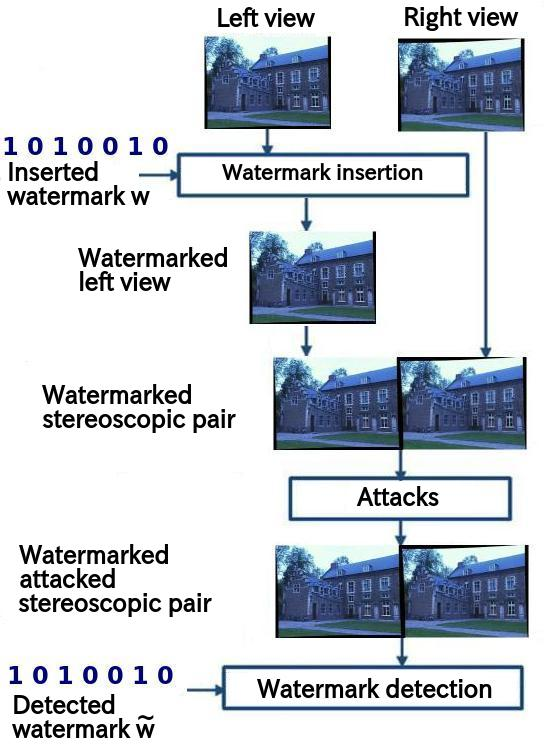
\includegraphics[width=0.8\textwidth]{./img/views_domain.jpeg}
\caption{\small{View-based watermarking workflow}}
\label{fig:view}
\end{figure}

\begin{figure}[h!]
\centering
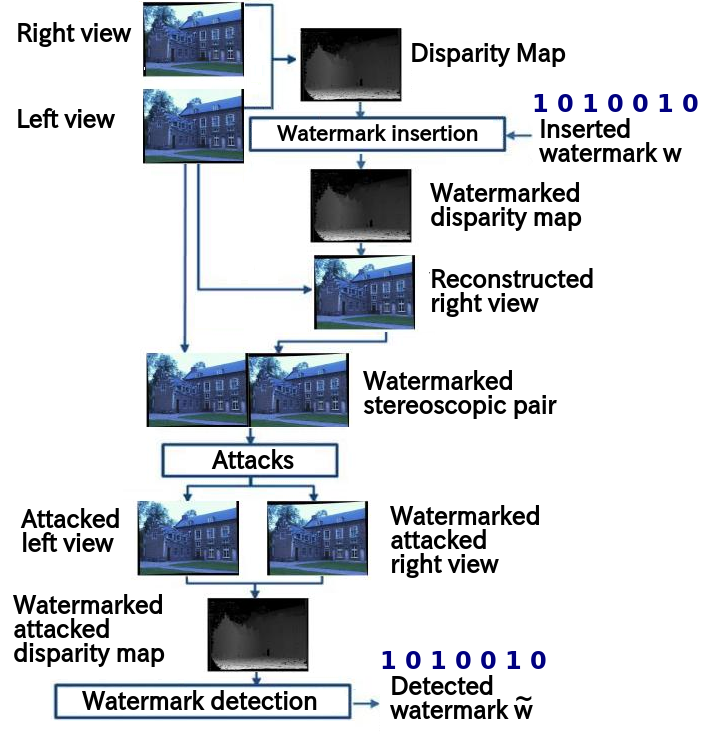
\includegraphics[width=1.05\textwidth]{./img/disparity_domain.png}
\caption{\small{Disparity-based watermarking workflow}}
\label{fig:disp}
\end{figure}


The predilection direction in the literature is represented by the view-based watermarking approaches, which are currently deployed for stereoscopic still images.\\ 
In this context disparity-coherent watermarking has been introduced,\cite{DOER}, to provide superior robustness against virtual view synthesis, as well as to improve perceived fidelity.\\
Disparity-coherence refers to the fact that a physical point of the captured scene should carry the
same watermark sample regardless of where it appears in the left/right view.\\
The advantages of producing disparity-coherent watermarks are two: first it produces pairs of stereoscopic views that are more in line with
what would naturally occur in reality and thereby yields less visual discomfort, second  disparity-coherent watermarks are expected to exhibit superior robustness against view synthesis, \cite{DOER}.\\
View synthesis consists in generating a virtual view in-between views that are available, e.g.the left and right views in stereo video. 

\subsection{Perception evaluation}

Perceptual impact can be defined as the imperceptibility of the embedded additional information in the watermarked content. This may signify either that the user is not disturbed by the artefacts induced by the watermark in the host document or that the user cannot identify any difference between the marked and the unmarked document.\\
The visual quality of the watermarked content in images and 2D video is usually objectively evaluated by five objective measures, namely, the PSNR, IF, NCC, SC, and SSIM \cite{METRICS}.\\

In this thesis the measures in \cite{QMETRICS} have been used to evaluate the quality of the watermarking technique in terms of human perception.\\
In Chaminda et al.'s study a Reduced-Reference
(RR) quality metric for color plus depth 3D video compression and transmission is proposed, using the extracted edge information of color plus depth map 3D video.\\ 
The work is motivated by the fact that the edges/contours of the depth map can represent different depth levels and this can be considered for measuring structural degradations. Since depth map boundaries are also coincident with the corresponding color image object boundaries, edge information of the color image and of the depth map is compared to obtain a quality index (structural degradation) for the corresponding color image sequence.\\
In order to quantify structural comparison, luminance comparison and contrast comparison parameters for the depth map and corresponding watermarked views, a modified version of the
commonly used SSIM metric is adopted:
\begin{equation}
Q_{Depth}(x,y) = [l(x,y)]^{\alpha} \cdot [c(x,y)]^{\beta} \cdot [\mathnormal{S}_{Depth}(x',y')]^{\gamma}
\end{equation}
where $l(x,y)$ and $c(x,y)$ are luminance and contrast comparisons performed on original depth maps and the ones computed after watermarking,
respectively, and $\mathnormal{S}_{Depth}(x',y')$  is the structural comparison between the gradient/edge maps of original and post-watermarking computed depth map images.\\
Then the overall depth map quality is calculated as
\begin{equation}
MQ_{Depth}(X,Y) = \frac{1}{M} \sum_{j=1}^{M}Q_{Depth}(x_{j},y_{j}).
\end{equation}
The SSIM-based quality index for the color image can be described as follows:
\begin{equation}
Q_{View}(x,y) = [l(x,y)]^{\alpha} \cdot [c(x,y)]^{\beta} \cdot [\mathnormal{S}_{View}(x',y')]^{\gamma}
\end{equation}
where $l(x,y)$ and $c(x,y)$ are luminance and contrast comparisons performed on original and watermarked views, respectively, and $\mathnormal{S}_{View}(x',y')$  is the structural comparison between the gradient/edge maps of the gradient maps of the corresponding original depth map and the watermarked views.\\
Hence, the overall color image quality is calculated as
\begin{equation}
MQ_{View}(X,Y) = \frac{1}{M} \sum_{j=1}^{M}Q_{View}(x_{j},y_{j}).
\end{equation}
As in \cite{QMETRICS}, the Sobel operator has been selected to obtain edge information (i.e., the binary edge mask) due to its simplicity and efficiency.\\

Finally the PSNR measure has been used to evaluate the quality of the watermarked videos and the quality of the compressed videos.\\
PSNR is the ratio between the maximum possible power of a signal and the power of corrupting noise that affects the fidelity of its representation; many signals have a very wide dynamic range, therefore PSNR is usually expressed in terms of the logarithmic decibel scale (dB). \\
For color images with three RGB values per pixel, the definition of PSNR is the following:
\begin{equation}
PSNR = 10 \cdot \log_{10}\bigg( \frac{MAX_{I}^2}{MSE}\bigg)
\end{equation}

\begin{equation}
MSE  = \frac{1}{3*MN} \sum_{i=0}^{M-1}\sum_{j=0}^{N-1}\Big(\mathbb{R} +\mathbb{G} + \mathbb{B}  \Big)
\end{equation}
with 
\begin{align}
\mathbb{R} &= [R_{I}(i,j)-R_{\tilde{I}}(i,j)]^{2} \\
\mathbb{G} &= [G_{I}(i,j)-G_{\tilde{I}}(i,j)]^{2} \\
\mathbb{B} &= [B_{I}(i,j)-B_{\tilde{I}}(i,j)]^{2}
\end{align}

where $I$ and $\tilde{I}$ are the $MxN$ reference image and the noisy approximation, respectively, and $MAX_{I}$ is the maximum possible pixel value of the image (when the pixels are represented using 8 bits per sample, this is 255).\\
For video sequence, the average value of all frames' PNSR value is computed.
Typical values for the PSNR in video compression and watermarking are between 30 and 50 dB.

\subsection{Robustness}
The robustness refers to the ability of detecting the watermark after applying some signal modifications
and malicious attacks on the marked content, such as spatial filtering, additive noise, geometric  transformations, lossy compression and, in stereoscopic context, view synthesis.

\subsubsection{Spatial filtering}
Linear filtering (such as blurring) and non-linear filtering (such as sharpening) are included in some image processing software: this operations remove from a signal some unwanted component or feature (Figure \ref{bl}).

\begin{figure}[h!]
\centering
\begin{subfigure}[]{0.4\textwidth}
\centering
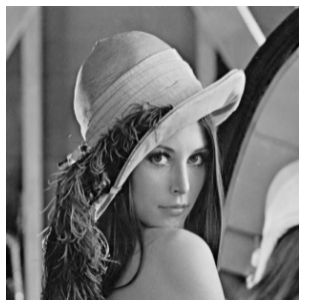
\includegraphics[width=0.8\textwidth]{./img/lena.png}
\caption{\small{Original image}}
\label{fig:lbO}
\end{subfigure}% 
\begin{subfigure}[]{0.4\textwidth}
\centering
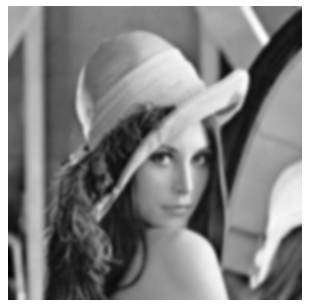
\includegraphics[width=0.8\textwidth]{./img/blur.png}
\caption{\small{Blurred image}}
\label{fig:blI}
\end{subfigure}% 
\caption{\small{Spatial filtering: blurring}\label{bl}}
\end{figure}

\subsubsection{Additive Noise}
The additive noise can be added to the content when applying some usual processing or when transmitting the signal over a communication channel during the broadcast (Figure \ref{noise}). 

\begin{figure}[h!]
\centering
\begin{subfigure}[]{0.4\textwidth}
\centering
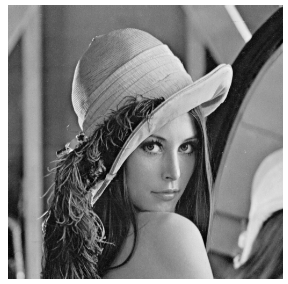
\includegraphics[width=0.8\textwidth]{./img/lena2.png}
\caption{\small{Original image}}
\label{fig:noise1}
\end{subfigure}% 
\begin{subfigure}[]{0.4\textwidth}
\centering
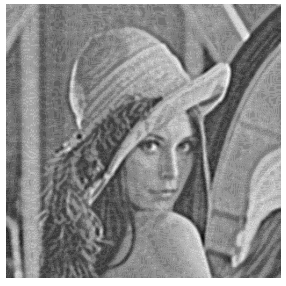
\includegraphics[width=0.8\textwidth]{./img/noise.png}
\caption{\small{Noised image}}
\label{fig:noise2}
\end{subfigure}% 
\caption{\small{Additive noise}\label{noise}}
\end{figure}

\subsubsection{Geometric distortions}
The geometric distortions include rotations, translations, spatial scaling, cropping and changes in aspect ratio (Figure \ref{geom}) they commonly occur during format changes.

\begin{figure}[h!]
\centering
\begin{subfigure}[]{0.4\textwidth}
\centering
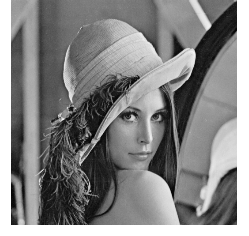
\includegraphics[width=0.8\textwidth]{./img/lena3.png}
\caption{\small{Original image}}
\label{fig:geom1}
\end{subfigure}% 
~ %add desired spacing between images, e. g. ~, \quad, \qquad,  etc.$  $
  %(or a blank line to force the subfigure onto a new line)
\begin{subfigure}[]{0.4\textwidth}
\centering
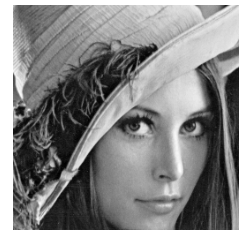
\includegraphics[width= 0.8\textwidth]{./img/crop.png}
\caption{\small{Cropped image}}
\label{fig:geom2}
  \end{subfigure}
\begin{subfigure}[]{0.4\textwidth}
\centering
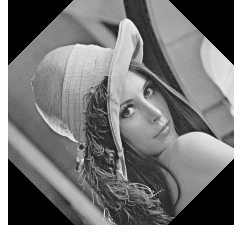
\includegraphics[width=0.8\textwidth]{./img/rot.png}
\caption{\small{Rotated image}}
\label{fig:geom3}
\end{subfigure}
\caption{\small{Geometric transformations}\label{geom}}
\end{figure}

\subsubsection{Lossy compression}
In video analysis, lossy compression is a common operation as it helps reduce resource usage, such as data storage space or transmission capacity.\newline  This process brings to a degradation of the image due to the compression ratio, thus affects the embedded watermark, as it removes the redundancy exploited in
watermarking schemes.\newline To prevent this problem a solution can be to improve the strenght of the embedded watermark.

\subsubsection{View synthesis}
Since in stereoscopic video context it is rather common practice to generate intermediate virtual views to adjust depth perception and since such view synthesis introduces non-rigid local geometric distortion that are not properly tackled by state-of-the art resynchronization mechanisms, stereo video watermarking strategies have to achieve robustness to synthetic view synthesis (Figure \ref{fig:vs}).\\

\begin{figure}[h!]
\centering
\begin{subfigure}[]{0.4\textwidth}
\centering
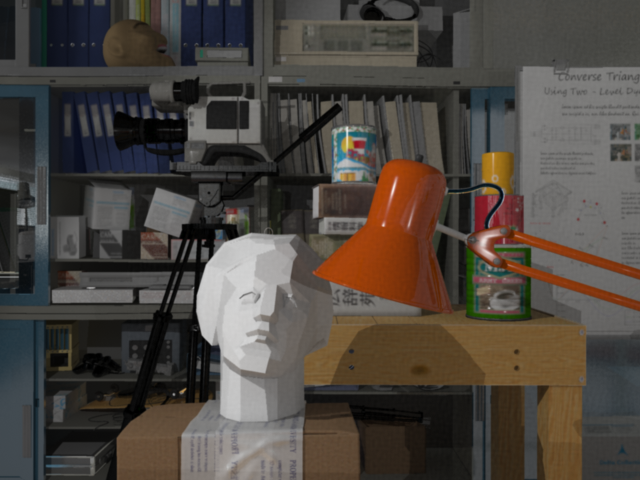
\includegraphics[width=0.8\textwidth]{./img/left_watermarked.png}
\caption{\small{Left image}}
\label{fig:vs1}
\end{subfigure}% 
~ %add desired spacing between images, e. g. ~, \quad, \qquad,  etc.$  $
  %(or a blank line to force the subfigure onto a new line)
\begin{subfigure}[]{0.4\textwidth}
\centering
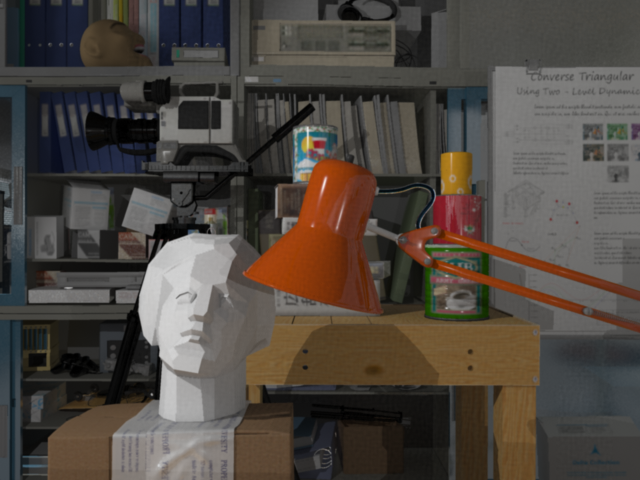
\includegraphics[width= 0.8\textwidth]{./img/right_watermarked.png}
\caption{\small{Right image}}
\label{fig:vs2}
  \end{subfigure}
\begin{subfigure}[]{0.4\textwidth}
\centering
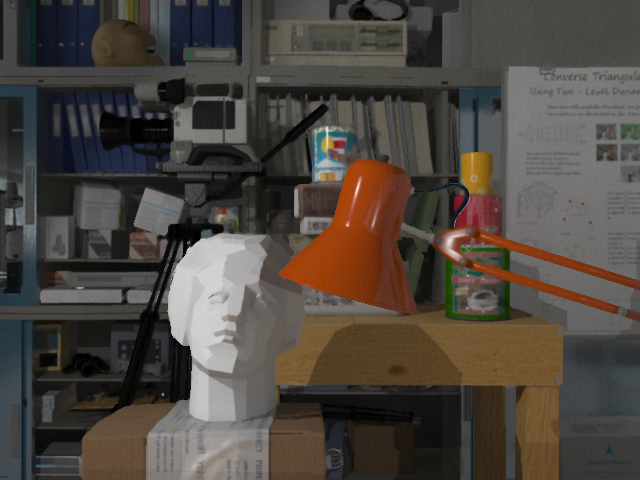
\includegraphics[width=0.8\textwidth]{./img/synth_view_watermarked.png}
\caption{\small{Synthetized view}}
\label{fig:vs3}
\end{subfigure}
\caption{\small{View synthesis}\label{fig:vs}}
\end{figure}



In this thesis a disparity-coherent watermarking algorithm has been implemented. It works in the frequency and spatial domain: a pseudo-random sequence of real numbers is embedded in a selected set of DFT coefficients of the left image then the reference watermark is spatially inserted in a disparity-coherent way in the right view.\\
It has shown good results in quality measure tests and roubustness test against view synthesis and compression.\\
An optimum criterion to verify if a given mark is present in an image is derived based on statistical decision theory, \cite{STAT}, allowing a robust watermark detection without resorting to the original uncorrupted image.\\








\chapter{Spatial disparity-coherent watermarking}
\markright{Spatial watermarking}
\label{spa}
\phantomsection
%\addcontentsline{toc}{chapter}{Spatial watermarking}



As said in the previous chapter, a number of works focused on how to incorporate depth information into the perceptual shaping process of the embedded watermark.\newline This process allows to achive disparity-coherence and makes sure that a physical point of the captured scene carries the same watermark sample regardless of where it appears in the left and right view.\newline

This process brings two advantages: it produces stereoscopic views more in line with reality, therefore yields less visual discomfort; and it is expected to have superior robustness against view synthesis.\newline

\section{Prior work} 

A prior work that is based on the disparity-coherent technique is the one carried on by Doerr et al in "Blind Detection for Disparity-Coherent
Stereo Video Watermarking" \cite{DOER2}.\newline
The watermark strategy  assumes that the key-seeded reference watermark pattern $w_{K}\textasciitilde N(0, 1)$ is embedded spatially in the left view and subsequently transferred to the right one.\newline
The watermark embedding and detection operations for the left view are therefore given by the conventional spread-spectrum equations:\newline
$$f_{l}^{w} = f_{l}+\alpha w_{K}$$
$$\rho(f_{l}+\epsilon\alpha w_{K},w_{K})= \frac{1}{wh}\sum_{x,y}(f_{l}(x,y)+\epsilon\alpha w_{K}(x,y))w_{K}(x,y)\approx\epsilon\alpha $$
where the superscript w indicates watermarked quantities, the subscript l (resp. r ) denotes quantities related to the left (resp. right) view, $\alpha > 0$ is the embedding strength, and w is normally distributed with zero mean and unit variance.\newline
The embedding strenght used in \cite{DOER2} to keep the embedding distortion imperceptible is $\alpha = 3$.\newline 

For the right view, the watermarking equation is the same, except that the watermark pattern $w_{K}$ is warped according to the depth information prior to insertion.

$$\forall(x,y) \in [1:w][1:h] f_{r}^{w}(x,y) = f_{r}(x,y)+\alpha w_{K}(x+d(x,y),y) = f_{r}+\alpha w_{K}^{d}(x,y) $$

The watermark detection on the right view relies on the computation of a horizontal cross-correlation array.\newline
$$\rho (f_{r}+\epsilon\alpha w_{K}^{d},w_{K}^{s})\approx\epsilon\alpha D_{s} $$
$$ \rho = \epsilon\alpha [D_{smin},..,D_{0},..,S_{smax}]$$
where $D_{s}$ is the proportion of pixels whose disparity value is exactly equal to s.\newline
The correlation array is then mapped into a scalar value in order to compare it with a threshold and to decide whether the tested content contains the watermark. Authors proposed three possible mapping functions:

$$\rho_{max}= \max_{s}\rho[s] $$
$$ \sum_{s}\rho[s] $$
$$ \sum_{|rho[s]|>\tau_{\rho}}|\rho[s]| $$

\section{ Gaussian-noise disparity-coherent watermarking} 

Based on the described technique, we propose a new spatial watermarking technique. \newline
For the spatial watermark its been taken under consideration the insertion of a Gaussian-noise reference watermark in an additive way.\newline
As in Doerr et al, the left view is processed in the conventional way, with spred-spectrum equations (riferimento all'equazione); the watermark is then warped according to the disparity value and inserted in the right view (rif all'eq), taking under consideration that the occluded zones shoudn't be processed.\newline
The added pattern and the reference images have the same size, so it should be noted that the warping process will generate a loss of marked pixel, due to the baseline's lenght.\newline
\begin{figure}[h!]
\centering
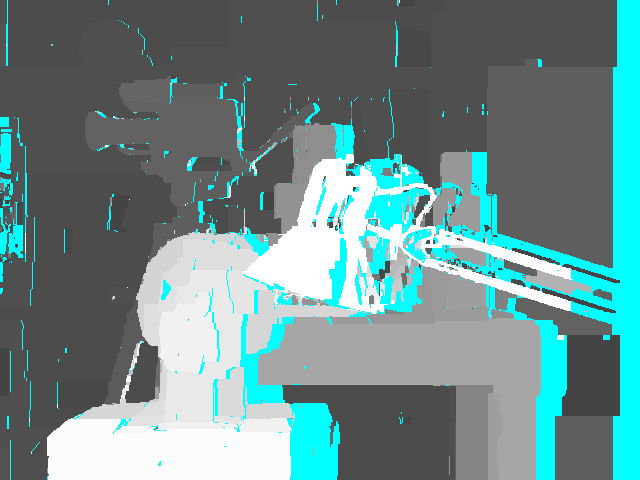
\includegraphics[width=0.5\textwidth]{./img/disp_left_to_right.png}
\caption{\small{Disparity left-to-right computed with KZ}}
\label{fig:kzdisplr}
\end{figure}
Since the disparity map and the occclusion map are usually not available, it needs to be estimated through the KZ algorithm, before the warping process.\newline
The embedding strenght is $\alpha=1$; it should be noted that this baseline watermarking framework could be enriched with conventional add-ons, e.g. perceptually modulate the embedding strength to better accommodate for the human visual system or canceling host interference for improved detection statistics.\newline

In the detection process, it has been used a conventional correlation-based detector for the left view (ref to eq).\newline 
On the other hand to detect the watermark in the right view two differet correlation-based strategies are proposed:
in the first strategy we computed the correlation value between the non-distorted watermark and the right view warped according to the right-to-left disparity, this way the priviously warped watermark is restored, even if there will be discontinuities due the occluded zones. In formula:
$$\rho((f_{r}+\epsilon\alpha w_{K}^{*})^{*},w_{K})= \frac{1}{wh}\sum_{x,y}(f_{r}(x,y)+\epsilon\alpha w_{K}^{*}(x,y))^{*}w_{K}(x,y)\approx\epsilon\alpha $$
where the superscript * indicates the warped mark/image.\newline

The second strategy is again a simple correlation-based detector, but the correlation value is computed between the right view and the warped watermark instead of the original one, based on the fact that the right view should contain this, rather than the reference pattern and that the reciever can compute the disparity map thats needed to warp the mark and perform the detection.

$$\rho(f_{r}+\epsilon\alpha w_{K}^{*},w_{K}^{*})= \frac{1}{wh}\sum_{x,y}(f_{r}(x,y)+\epsilon\alpha w_{K}^{*}(x,y))w_{K}^{*}(x,y)\approx\epsilon\alpha $$

To illustrates the performance of the binary classifier system as its discrimination threshold is varied it has been drawn the corresponding ROC curve.\newline  The ROC curve is a representation of the sensitivity as a function of fall-out.\newline  The curve is created by plotting the true positive rate (TPR) against the false positive rate (FPR) at various threshold settings.\newline The true-positive rate is also known as sensitivity and the false-positive rate is also known as the fall-out.\newline  

\begin{figure}[h!]
\centering
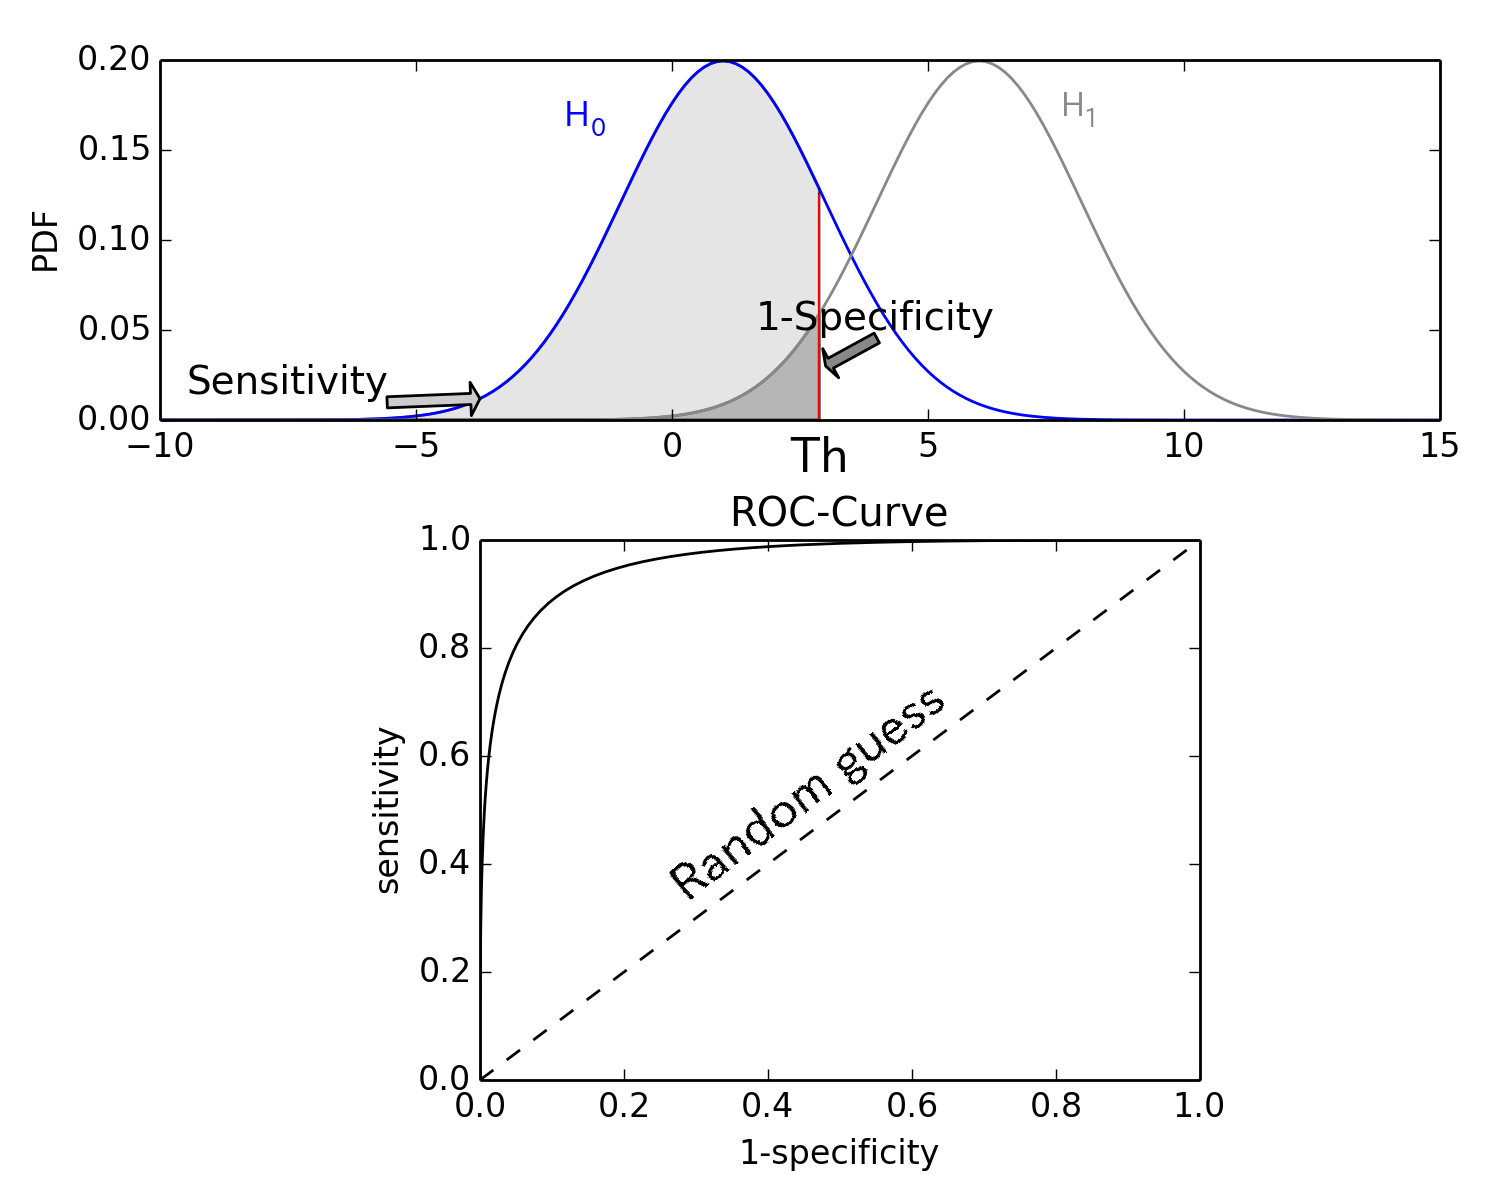
\includegraphics[width=0.7\textwidth]{./img/roc.png}
\caption{\small{Top: Probability density functions for two distributions. Bottom: corresponding ROC-curve.}}
\label{fig:roc}
\end{figure}

\begin{figure}[h!]
\centering
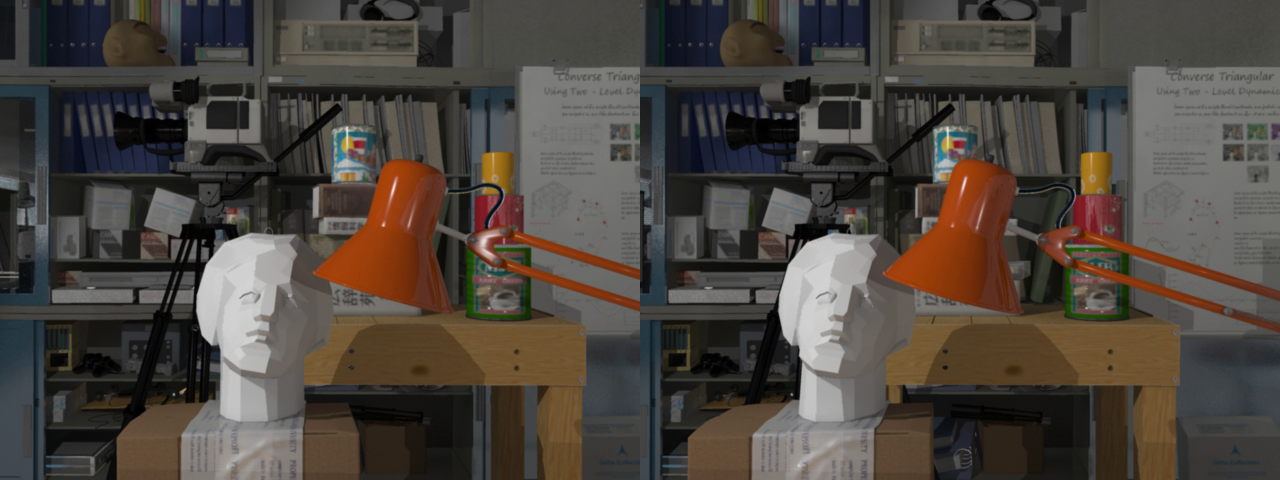
\includegraphics[width=1\textwidth]{./img/marked_1_gauss.png}
\caption{\small{Stereo image marked with spatial algorithm with power equal to 1.}}
\label{fig:gauss1}
\end{figure}
\begin{figure}[h!]
\centering
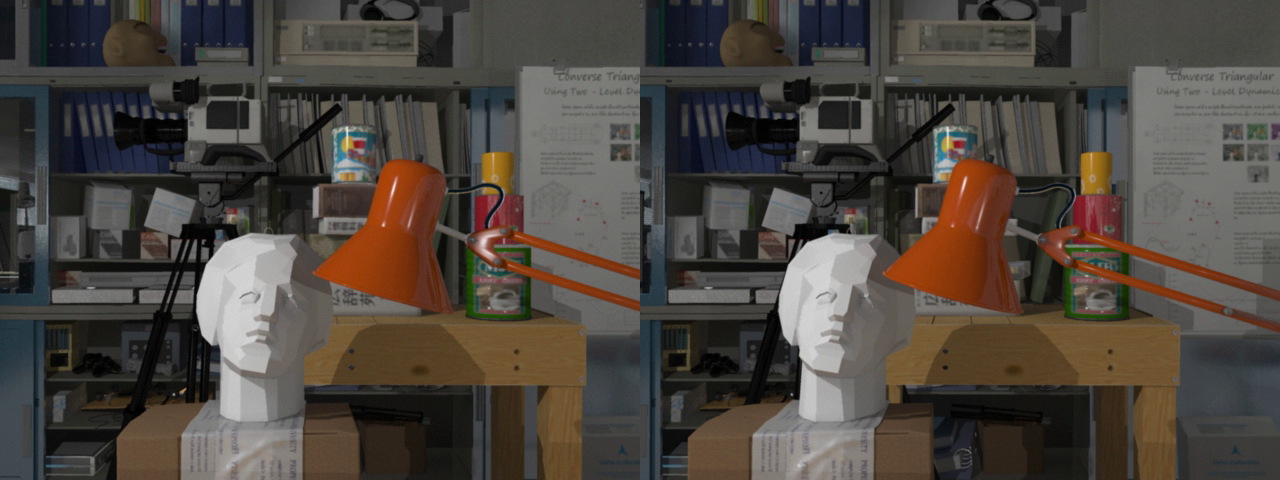
\includegraphics[width=1\textwidth]{./img/marked_3_gauss.png}
\caption{\small{Stereo image marked with spatial algorithm with power equal to 1}}
\label{fig:gauss3}
\end{figure}
  
As said before the disparity-coherent watermarking have the ability to detect the embedded watermark in synthetized views: to performe the detection on a random right view, that might be synthetized, the detector will need to calculate the disparity map between the analyzed view and the recieved left, and warp it accordingly, to recompose the original watermark.\newline 
There is then a tight bond between the watermarking process and the evaluation of the disparity maps; with the graph-cuts algorithm it's possible to compute accurate maps and to know the occluded zones.

\chapter{Frequency disparity-coherent watermarking}
\markright{Frequency disparity-coherent watermarking}
\label{dft}
\phantomsection

Now we proposed a variant of the described watermarking process, which works in the frequency domain.

\section{Watermark in Fourier domain}

The strategy is based on the technique presented by Piva et al in "Improving DFT Watermarking robustness through optimum detection and synchronisation" \cite{PIVA}, where a watermarking algorithm for digital images operating in the frequency domain is presented: the method embeds a pseudo-random sequence of real numbers in a selected set of DFT coefficients of the image. Moreover, a synchronisation pattern is embedded into the watermarked image, to cope with geometrical attacks, like resizing and rotation. After embedding, the watermark is adapted to the image by exploiting the masking characteristics of the Human Visual System, thus ensuring the watermark invisibility.\newline
\begin{figure}[h!]
\centering
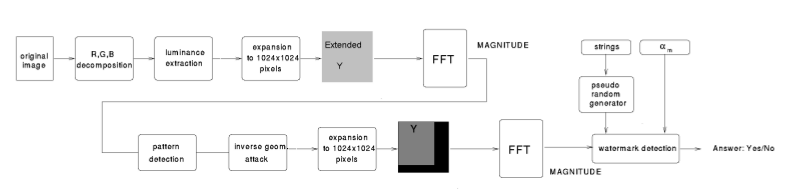
\includegraphics[width=1\textwidth]{./img/blocchi.png}
\caption{\small{Piva et. al watermarking workflow}}
\label{fig:blocchi}
\end{figure}

For the stereo watermarking task this process has been simplified and cut to the basic frequency watermaking.

\subsection{Watermark embedding}

In \cite{PIVA} the watermark is embedded in a subset of DFT coefficients of the luminance $Y$.\newline Since a traslation of the scene will only change the phase values of the DFT, leaving unaltered the magnitude values, the watermak only concernes the latter, to achieve robustness against image traslation.\newline
To garantee a blind detection system the number and position of the coefficient are fixed a priori: based on the size of the image to watermark, the coefficient are choosen in the medium frequencies of the spectrum to achieve a compromise between robustness and invisibillity.\newline 
The watermark embedding rule is the following:
\begin{equation}\label{eq:wat}
y_{i}^{'} = y_{i}+\alpha m_{i}y_{i} 
\end{equation}

where $y_{i}^{'}$ represents the watermarked DFT magnitude coefficient, $y_{i}$ the corresponding original, $m_{i}$ is a sample of the watermark sequence, and $\alpha$ is the watermark energy.\newline
The inverted DFT is then applied to obtain the watermarked luminance $Y^{'}$.

\subsection{Watermark detection}

To determine if a given image luminance $Y$ either embedds or not the reference watermark in \cite{PIVA} a threshold-based detection is used.\newline
The luminance of the received image is extracted and its DFT trasform is computed; from the obtained magnitude matrix the right coefficents can be selected since their positions are known as said above.\newline
Knowing the seed (in the shape of two strings, one numeric one alphanumeric) the watermark can be reproduced.\newline

To verify if the selected coefficients have been altered by means of the watermark it is used a statistical decision theory: two hypotheses are defined, the image contains the reference watermark (hypotheses $H_{1}$) or the image does not contain this mark (hypotheses $H_{0}$). Relying on Bayes theory of hypothesis testing, the optimum criterion to test H1 versus H0 is minimum Bayes risk; the test function results to be the likelihood ratio function L that has to be compared to a threshold:\newline
\begin{itemize}
\item if $L > \lambda$ ,  the watermark $m^{*}$ is present;
\item if $L < \lambda$ , the watermark  $m^{*}$ is absent.
\end{itemize}

To choose a proper threshold, it has been chosen to fix a constraint on the maximum false positive probability and the optimum decoder is designed refferring to the Neyman-Pearson criterion, as: \newline

$$ L(y)=\sum_{i=0}^{N-1} [-\beta ln(1+\alpha_{m}m_{i}^{*})]+\sum_{i=0}^{N-1}[-(\frac{y_{i}}{\alpha_{i}(1+\alpha_{m}m_{i}^{*})}))^{\beta_{i}}+(\frac{y_{i}}{\alpha_{i}})^{\beta_{i}}] $$
and
$$\lambda=3.3\sqrt{2\sum_{i=0}^{N-1}[\frac{[(1+\alpha_{m}m_{i}^{*})^{\beta_{i}}]}{(1+\alpha_{m}m_{i}^{*})^{\beta_{i}}}]} + \sum_{i=0}^{N-1}\{\frac{[(1+\alpha_{m}m_{i}^{*})^{\beta_{i}}-1]}{(1+\alpha_{m}m_{i}^{*})^{\beta_{i}}}\} - \sum_{i=0}^{N-1}[\beta_{i}ln(1+\alpha_{m}m_{i}^{*})]$$

In ()  $m^{*} = \{ m^{*}_{i} \} i= 0,1,...N-1$ is the watermark, $\alpha_{m}$ the mean watermark energy, $\alpha_{i}$ and $\beta_{i}$ are statistic parameters describing the probability density function shape of the magnitude of the watermarked DFT coefficients $y_{i}$.\newline 
The values of this parameters are choosen by means of Maximum Likelihood criterion, based on the the fact that the coefficients belonging to small
sub-regions of the spectrum are characterised by the same statistic parameters and follows a Weibull distribution, modeled as:
$$ f(y_{i}) = \frac{\beta}{\alpha}(\frac{y_{i}}{\alpha})^{\beta-1}\exp\{-(\frac{y_{i}}{\alpha})^{\beta}\}$$
In summary, the detection process can be decomposed in the following steps:
\begin{itemize}
\item generation of the watermark $m^{*}$;
\item estimation of the parameters $\alpha,\beta$ into the regions composing the watermarked area of the spectrum;
\item computation of $L(y)$ and $\lambda$ ;
\item comparison between $L(y)$ and $\lambda$ ;
\item decision.
\end{itemize}

The decoder can detect the watermark presence also in highly degraded images. In particular, the system is robust to sequences of different attacks, such as rotation, resizing, and JPEG compression, or such as cropping, resizing and median filtering.

\section{Stereo watermarking embedding}

For the stero-marking process its been taken under consideration a 512x512 subset of pixel of the image, in particular we focused in marking the part of the scene which is common to both the left and right view.

\begin{figure}[h!]
\centering
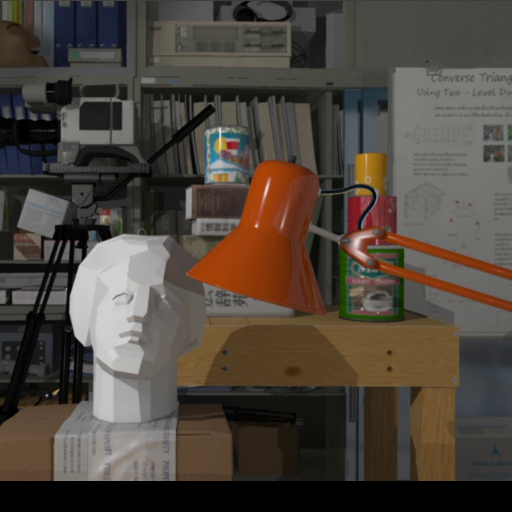
\includegraphics[width=0.5\textwidth]{./img/squared.png}
\caption{\small{Cropped image to watermark}}
\label{fig:cropped}
\end{figure}

The left view is then processed with the algorithm discribed above.\newline 

In order to mark the left and right view with the same watermark, but in a disparity-coherent way a study on the left marking process has been conducted.
The $NXM$ left image $l$ can be written as a function of its DFT transform $L$:
$$ l =  \frac{1}{MN}\sum\sum(|L(u,v)|)\exp\{\phi (u,v)\} \exp\{+j2\pi(\frac{ux}{M}\frac{vy}{N})\}  $$
The marking process alters the DFT coefficients according to the Equation in \ref{eq:wat}
which can be written by:
$$ l_{w} = \frac{1}{MN}\sum\sum(|L(u,v)| + \alpha|L(u,v)||w|)\exp\{j(\phi_{L}+\phi_{w})\}\exp\{+j2\pi(\frac{ux}{M}\frac{vy}{N})\} $$
the signal alteration is therefore given by:
$$ \alpha|L||w|exp\{j(\phi_{L}+\phi{w})\} $$ 
where $|w|$ is the magnitude of the watermark, $\phi_{L}$ is the phase of the left view and $ \phi_{w}$ the phase of the watermark which takes value in \{0,\pi\}.

To obtain the same additive multiplicative alteration on the right view coefficients we created the watermark ad-hoc with the following formula: 
$$ \alpha|R^{*}||w|exp\{j(\phi_{L}+\phi{w})\} $$ 
the subscript * indicates that the right image has been warped according to he right-to -left disparity to have the same phase of the left image, and generte the correct mark.
The created mark is the brought in then spatial domain and warped according to the left-to right disparity previous to spatial insertion in the right view.

The complete formula can then be written as: 
$$ l_{w} = l + \frac{1}{MN}\sum\sum(\alpha|L(u,v)||w|\exp\{j(\phi_{L}+\phi_{w})\})\exp\{+j2\pi(\frac{ux}{M}\frac{vy}{N})\} $$
$$ r_{w} = r + \frac{1}{MN}\sum\sum(\alpha|R(u,v)^{*}||w|\exp\{j(\phi_{L}+\phi_{w})\})^{**}\exp\{+j2\pi(\frac{ux}{M}\frac{vy}{N})\} $$

The subscript ** indicates the warping according to the left-to-right disparity.

\begin{figure}[h!]
\centering
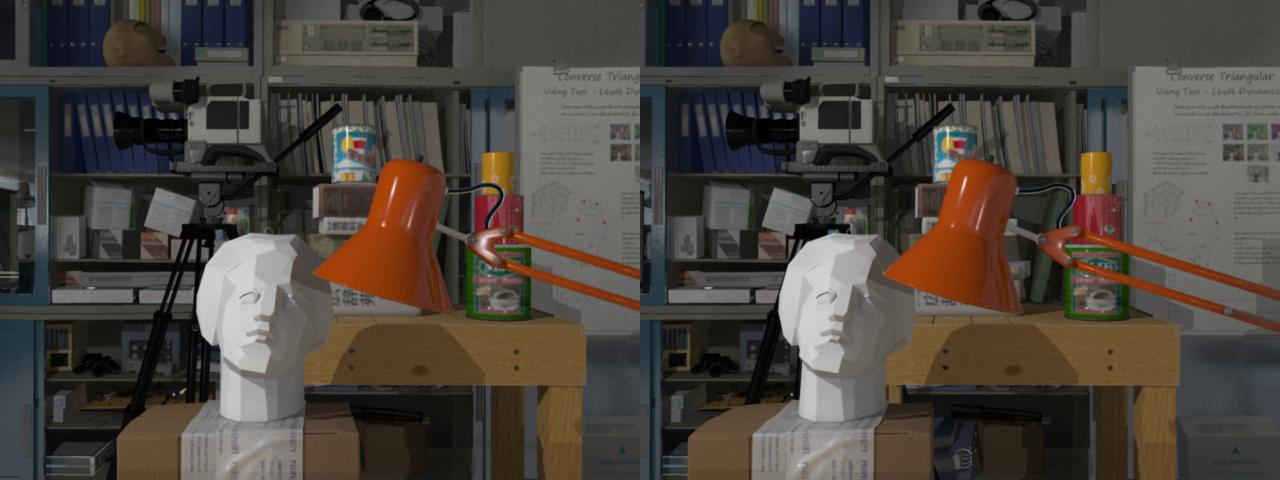
\includegraphics[width=1\textwidth]{./img/marked_03_DFT.png}
\caption{\small{stereo image marked with DFT algorithm with power equal to 0.3}}
\label{fig:dft03}
\end{figure}
\begin{figure}[h!]
\centering
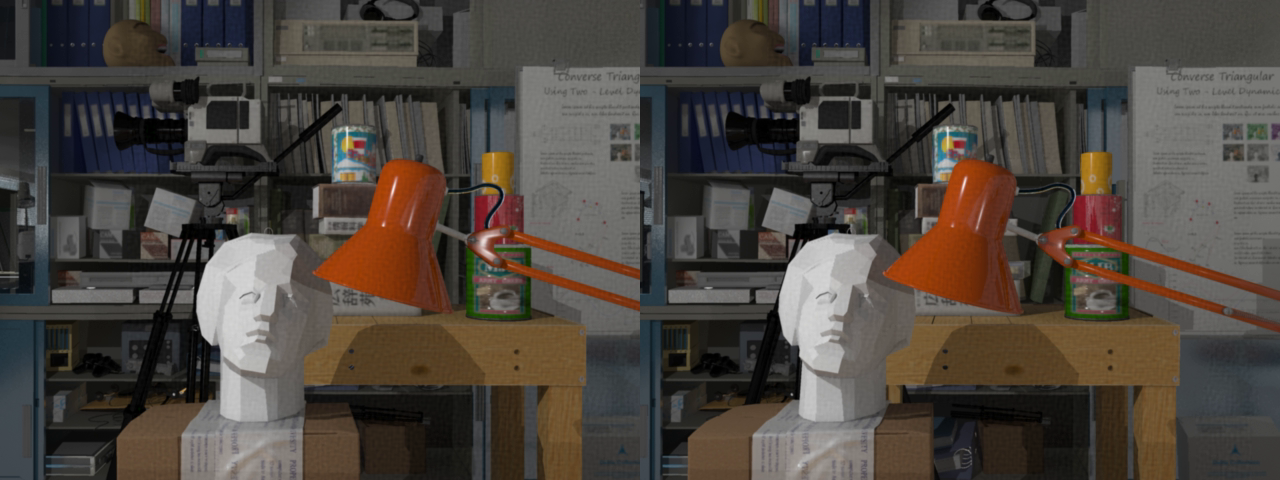
\includegraphics[width=1\textwidth]{./img/marked_05_DFT.png}
\caption{\small{Stereo image marked with DFT algorithm with power equal to 0.5}}
\label{fig:dft05}
\end{figure}
\begin{figure}[h!]
\centering
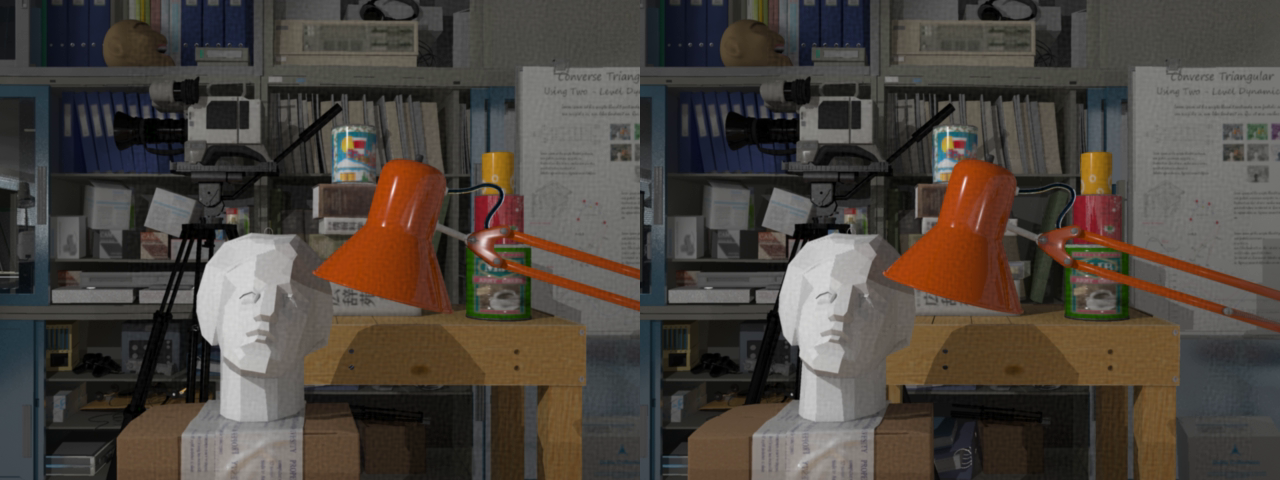
\includegraphics[width=1\textwidth]{./img/marked_06_DFT.png}
\caption{\small{Stereo image marked with DFT algorithm with power equal to 0.6}}
\label{fig:dft06}
\end{figure}
\begin{figure}[h!]
\centering
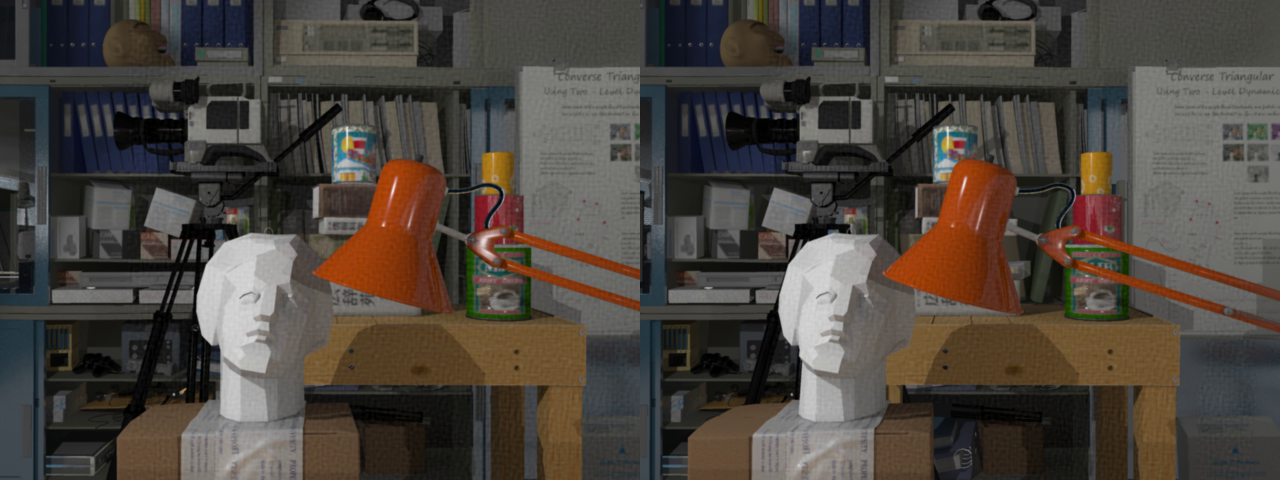
\includegraphics[width=1\textwidth]{./img/marked_07_DFT.png}
\caption{\small{Stereo image marked with DFT algorithm with power equal to 0.7}}
\label{fig:dft07}
\end{figure}
\section{Stereo detection algorithm}

The detection of the watermark is performed with the detector implemented by Piva et al.\newline

As for the embedding process, the algorithm is applied to the left view without changes, meanwhile, some adaptations are needed for the right view detection.\newline

First the detection algorithm computes the right-to-left disparity, then the right view is warped accordingly to ricreate the phase of the inserted watermark; to mantain the correctt phase the occluded zones are filled with the pixels of the recieved left view (taking under consideration that this little amount of image's pixel would not influence the detection).\newline
The created image is then processed by the threshold-based detection algorithm.\newline 

\begin{figure}[h!]
\centering
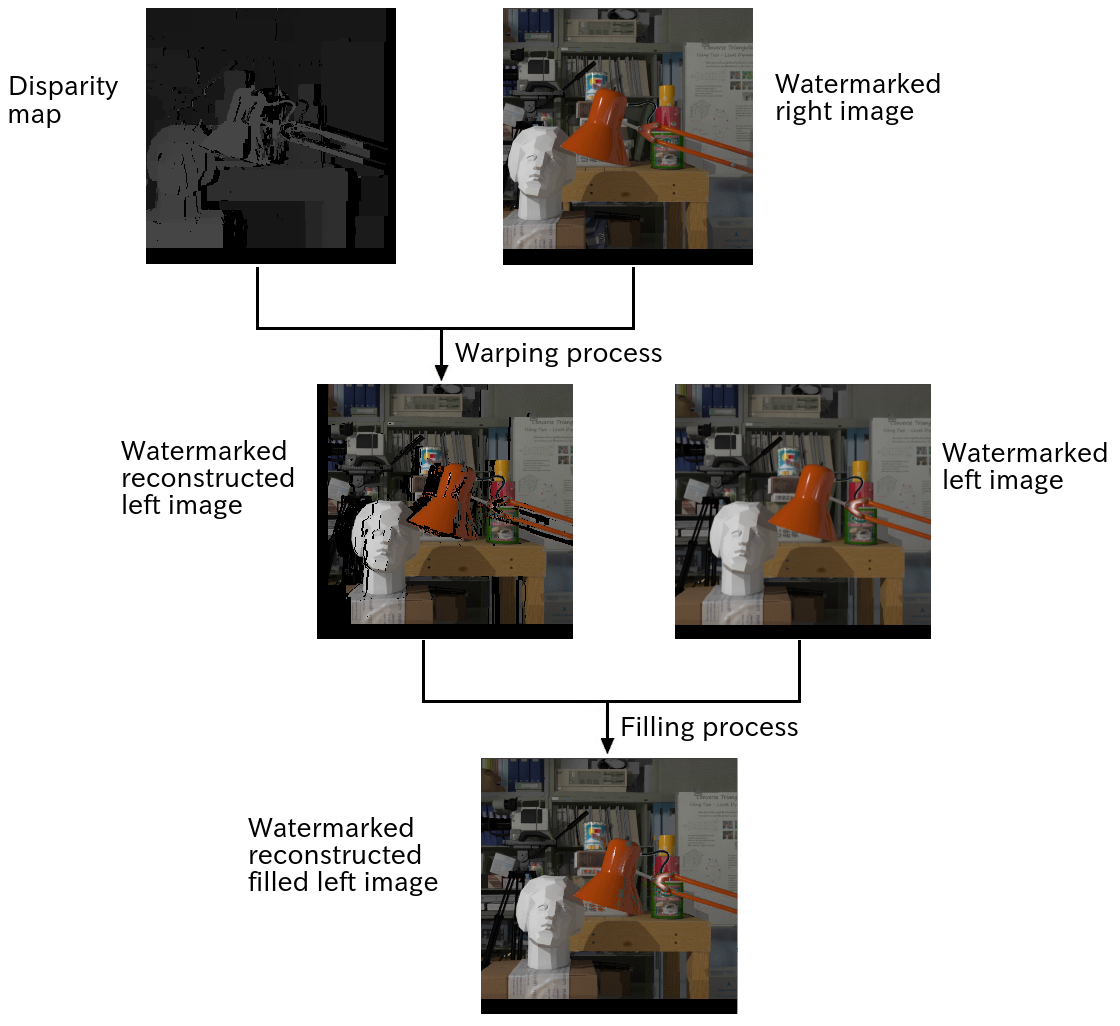
\includegraphics[width=1\textwidth]{./img/detection_workflow.png}
\caption{\small{Detection workflow}}
\label{fig:detflow}
\end{figure}


\chapter{Conclusions}
\markright{Conclusions}
\phantomsection
%\addcontentsline{toc}{chapter}{Conclusions}


\phantomsection
\addcontentsline{toc}{chapter}{Bibliografia}
\bibliographystyle{plain}
\bibliographystyle{plain}
\begin{thebibliography}{99}

\bibitem{MED} P.-L. Chang, D. Stoyanov, A. Davison, and P. E. Edwards, Real-time
dense stereo reconstruction using convex optimisation with a cost-volume for image-guided robotic surgery, Proc. MICCAI,2013

\bibitem{MED2}Bhayani SB, Andriole GL.,Three-Dimensional (3D) Vision: Does It Improve Laparoscopic Skills? An Assessment of a 3D Head-Mounted Visualization System. Reviews in Urology. 2005;7(4):211-214


\bibitem{TRACK}Muñoz-Salinas, Rafael, Eugenio Aguirre, and Miguel García-Silvente, People detection and tracking using stereo vision and color. Image and Vision Computing 25.6 (2007): 995-1007

\bibitem{PG} Point Grey Stereo Vision Introduction and Applications \url{http://www.ptgrey.com/support/downloads/10353}


\bibitem{GAME} \url{http://www.nvidia.com/docs/IO/66368/Top-10-3D-Games-by-APC.PDF}


\bibitem{BP} Radhakrishnamurthy, H.Ch. et al.: Stereo Vision System for A Bin Picking Adept Robot, Malaysian Journal of Computer Science. Vol. 20, No. 1, 2007, pp. 91 - 98 

\bibitem{DEVICE} A Beginner's Guide to Shooting Stereoscopic 3D \\ \url{http://www.dashwood3d.com/blog/beginners-guide-to-shooting-stereoscopic-3d/}

\bibitem{BUMBLE} \url{https://www.ptgrey.com//bumblebee2-firewire-stereo-vision-camera-systems}

\bibitem{AUTO}\url{http://www.autonomoustuff.com/stereo-vision.html}

\bibitem{SV}Stefano Mattoccia, Stereo Vision: Algorithms and Applications
\url{www.vision.deis.unibo.it/smatt}

\bibitem{SV2}P. K. Sinha, Image Acquisition and Preprocessing for Machine Vision Systems, SPIE Press, Bellingham (2012)

\bibitem{ZISS}Hartley, R. and Zisserman, A. 2000. Multiple view geometry in computer vision, Cambridge University Press: Cambridge, UK


\bibitem{KZ}Vladimir Kolmogorov, Pascal Monasse, and Pauline Tan, Kolmogorov and Zabih’s Graph Cuts Stereo Matching Algorithm, Image Processing On Line, 4 (2014), pp. 220–251. \url{http://dx.doi.org/10.5201/ipol.2014.97}

\bibitem{ALPHA}D. Batra, P. Kohli, Making the right moves: guiding alpha-expansion using local primal-dual gaps, in: IEEE Conference on Computer Vision and Pattern Recognition (CVPR), 2011

\bibitem{3D} \url{http://www.sky.com/shop/__PDF/3D/Basic_Principles_of_Stereoscopic_3D_v1.pdf}

\bibitem{3D2} \url{http://www.techradar.com/news/television/active-shutter-vs-passive-3d-tv-which-is-best-958717}

\bibitem{COX}Cox, Ingemar J., et al. "Secure spread spectrum watermarking for multimedia." Image Processing, IEEE Transactions on 6.12 (1997): 1673-1687

\bibitem{COX1}Cox I, Miller M, Bloom J (2002) Digital watermarking. Morgan Kaufmann, San Mateo


\bibitem{COX2} Cox I, Miller M, Bloom J (2002) Digital watermarking. Morgan Kaufmann, San Mateo

\bibitem{SH} Shannon CE (1958) Channel with side information at the transmitter. IBM Journal of Research and Development 2(4):289–293

\bibitem{EG} Eggers JJ, Bäuml R, Tzschoppe R, Girod B (2003) Scalar Costa scheme for information embedding. IEEE Trans Signal Process 51(4)

\bibitem{COSTA} Costa MHM (1983) Writing on dirty paper. IEEE Trans Inf Theory IT-29(3):439–441


\bibitem{16}Dong-Choon H, Kyung-Hoon B, Eun-Soo K (2003) Real-time stereo image watermarking using discrete cosine transform and adaptive disparity maps. Multimedia Systems Appl VI, Proc SPIE 5241:233

\bibitem{17}Dong-Choon H, Kyung-Hoon B, Eun-Soo K (2003) Stereo image watermarking scheme based-on discrete wavelet transform and adaptive disparity estimation. Mathematics of data/image coding, compression, and encryption, with applications. Conference no. 6, San Diego

\bibitem{18}Kumar S, Raman B, Thakur M (2009) Real coded genetic algorithm based stereo image watermarking. IJSDA Int J Secure Digit Inf Age 1(1)

\bibitem{19}Bhatnager G, kumar S, Raman B, Sukavanam N (2009) Stereo coding via digital watermarking. J Electron Imaging 18(3)

\bibitem{20}Campisi P (2008) Object-oriented stereo image digital watermarking. J Electron Imaging 17(4):043024

\bibitem{21}Yu M, Wang A, Luo T, Jiang G, Li F, Fu S (2011) New block relationship based stereo image watermarking algorithm. In: The sixth international conference on systems and networks communications, ICSNC 2011, pp 171–174 (October 2011)

\bibitem{22}Zhang Z, Zhu Z, Xi L (2007) Novel scheme for watermarking stereo video. Int J Nonlinear Sci 3(1):74–80

\bibitem{QIM}Hasnaoui M, Belhaj M, Mitrea M, Prêteux F (2011) mQIM principles for MPEG-4 AVC watermarking, SPIE Photonics West 2011 (January 2011)

\bibitem{QIM1}Belhaj M, Mitrea M, Duta S, and Preteux F (2010) MPEG-4 AVC robust video watermarking based on QIM and perceptual masking. In: International conference on communication, Bucharest (June 2010)

\bibitem{METRICS}Joshi, Madhuri A., et al. Image and Video Compression: Fundamentals, Techniques, and Applications. CRC Press, 2014

\bibitem{QMETRICS} Hewage, Chaminda TER, and Maria G.Martini, Edges-based reduced-reference quality metric for 3D video compression and transmission. Selected Topics in Signal Processing, IEEE Journal of 6.5 (2012): 471-482.



\bibitem{DOER}Faridul, Hasan Sheikh, Gwenaël Doërr, and Séverine Baudry, Disparity estimation and disparity-coherent watermarking. IST/SPIE Electronic Imaging. International Society for Optics and Photonics, 2015.


\bibitem{STAT}L. Scharf, Statistical Signal Processing: detection,
estimation, and time series analysis, Add. Wesley,
1991.






\end{thebibliography}
\clearpage
\thispagestyle{empty}
\end{document}